\documentclass[a4paper,12pt]{article}
\usepackage[utf8]{inputenc}
\usepackage[spanish]{babel}
\usepackage{amsmath}
\usepackage{graphicx}
\usepackage{float}
\usepackage{geometry}
\usepackage{titlesec}
\usepackage{caption}
\usepackage{subcaption}

\geometry{left=2.5cm, right=2.5cm, top=2.5cm, bottom=2.5cm}

\titleformat{\section}{\normalfont\Large\bfseries}{S\thesection}{1em}{}

\title{Informe de Simulación de Sistema de Colas M/M/c/K}
\author{}
\date{}

\begin{document}

\maketitle

\section{Introducción}

Este proyecto tiene como objetivo simular un sistema de atención de solicitudes representado por un modelo de colas M/M/c/K. Dicho sistema modela la llegada de solicitudes a un servidor con múltiples hilos (o servidores), una cola finita y una política de servicio FIFO.

\subsection*{Objetivos y metas}

\begin{itemize}
    \item Evaluar el rendimiento del sistema bajo diferentes configuraciones de parámetros clave.
    \item Medir métricas como porcentaje de solicitudes rechazadas, tiempo promedio de respuesta y uso del servidor.
    \item Estudiar cómo varían estas métricas al modificar la tasa de llegada (\( \lambda \)), tasa de servicio (\( \mu \)), número de hilos y tamaño de la cola.
\end{itemize}

\subsection*{Variables que describen el problema}

\begin{itemize}
    \item \( \lambda \): tasa de llegada de solicitudes.
    \item \( \mu \): tasa de servicio por hilo.
    \item \( c \): número de hilos disponibles.
    \item \( K \): tamaño máximo de la cola de espera.
\end{itemize}

\section{Detalles de Implementación}

La simulación fue implementada en Python utilizando un enfoque basado en eventos discretos. Se desarrolló una clase que modela el sistema con su cola de eventos, tiempos de servicio y control de estados.

Se realizaron simulaciones independientes variando un parámetro a la vez, manteniendo los demás fijos. Cada experimento corrió durante un tiempo simulado de 1000 unidades, tiempo suficiente para observar un comportamiento representativo del sistema.

\section{Resultados y Experimentos}

\subsection*{Hilos vs Porcentaje de Rechazo}

Se observó que al incrementar el número de hilos disponibles, el porcentaje de solicitudes rechazadas disminuye drásticamente, especialmente entre 1 y 5 hilos. Más allá de este valor, la mejora se estabiliza.

\begin{figure}[H]
    \centering
    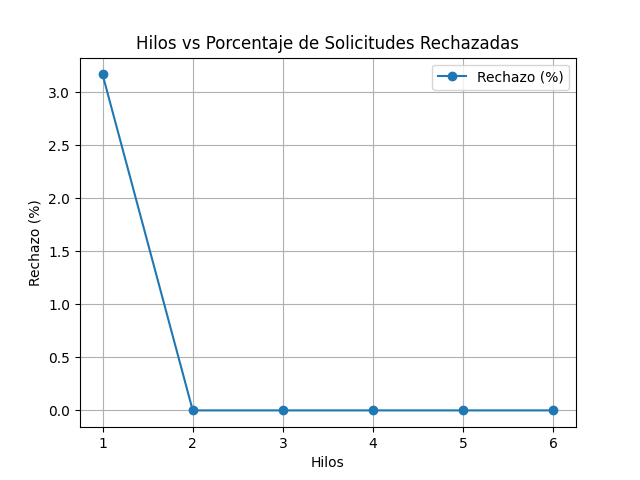
\includegraphics[width=0.7\textwidth]{../graphs/threads_vs_rejection.png}
    \caption{Porcentaje de solicitudes rechazadas en función del número de hilos}
\end{figure}

\subsection*{Tamaño de la cola vs Tiempo de respuesta y Rechazo}

Se encontró que una cola más grande reduce el porcentaje de rechazos, pero también aumenta el tiempo de respuesta promedio debido al mayor número de solicitudes en espera.

\begin{figure}[H]
    \centering
    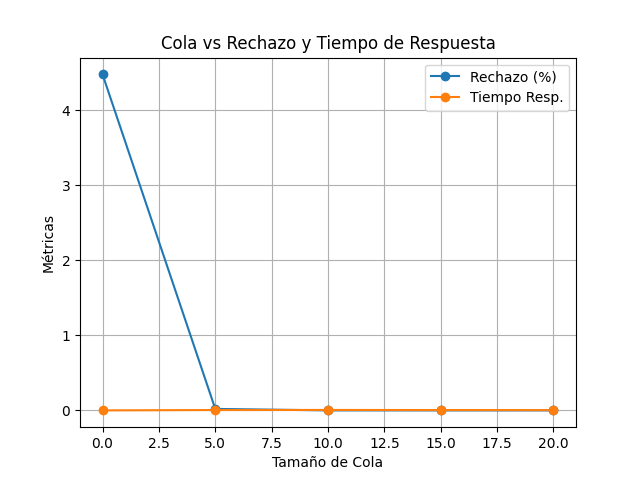
\includegraphics[width=0.7\textwidth]{../graphs/queue_vs_response.png}
    \caption{Tiempo de respuesta y rechazos según tamaño de la cola}
\end{figure}

\subsection*{Tasa de llegada \( \lambda \) vs Uso y Rechazo}

A medida que se incrementa \( \lambda \), el uso del servidor aumenta hasta llegar al 100\%, momento en que las solicitudes empiezan a ser rechazadas por falta de capacidad.

\begin{figure}[H]
    \centering
    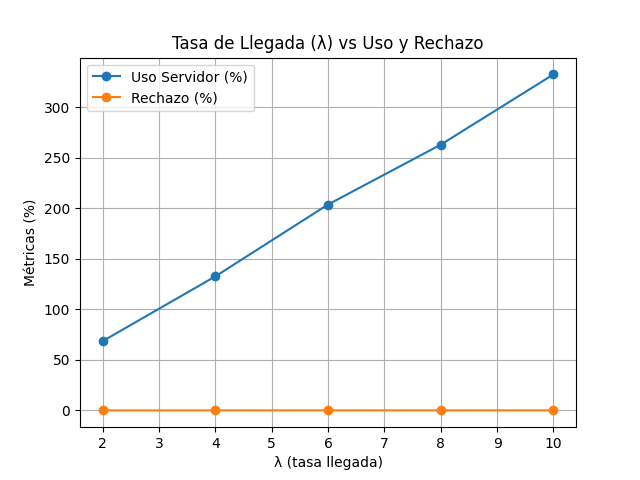
\includegraphics[width=0.7\textwidth]{../graphs/lambda_vs_metrics.png}
    \caption{Relación entre tasa de llegada, uso del servidor y rechazo}
\end{figure}

\subsection*{Tasa de servicio \( \mu \) vs Uso y Rechazo}

Aumentar la tasa de servicio reduce el tiempo en que cada solicitud permanece en el sistema, lo cual disminuye el rechazo y mejora el uso del servidor.

\begin{figure}[H]
    \centering
    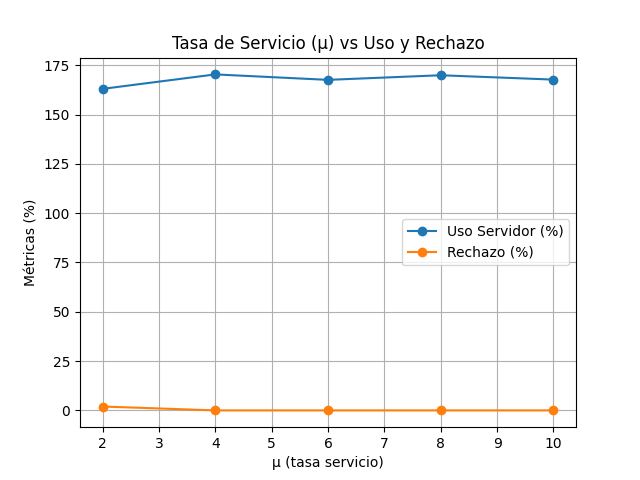
\includegraphics[width=0.7\textwidth]{../graphs/mu_vs_metrics.png}
    \caption{Relación entre tasa de servicio y desempeño del sistema}
\end{figure}

\subsection*{Hipótesis validadas}

\begin{itemize}
    \item Aumentar hilos mejora el rendimiento, con rendimientos decrecientes después de cierto punto.
    \item El tamaño de cola permite reducir rechazos pero penaliza la latencia.
    \item Cuando \( \lambda > c\mu \), el sistema entra en saturación rápidamente.
\end{itemize}

\section{Modelo Matemático}

El modelo utilizado es una cadena de Markov de nacimiento y muerte con parámetros:

\begin{itemize}
    \item Llegadas Poisson con tasa \( \lambda \).
    \item Servicios exponenciales con tasa \( \mu \) por hilo.
    \item \( c \) servidores paralelos.
    \item Capacidad total del sistema: \( c + K \).
\end{itemize}

\subsection*{Supuestos}

\begin{itemize}
    \item Las llegadas y servicios son independientes.
    \item Política de servicio FIFO.
    \item Todos los servidores son idénticos.
\end{itemize}

Los resultados de la simulación están alineados con la teoría de colas, validando el modelo implementado.

\section{Conclusiones}

La simulación permitió analizar en profundidad los efectos de variaciones en los parámetros del sistema. Se validaron hipótesis clave de la teoría de colas y se comprendió el comportamiento de un sistema bajo diferentes configuraciones de carga.

Los gráficos comparativos permiten tomar decisiones informadas sobre arquitectura de sistemas en escenarios reales.

\end{document}